% !TeX root = ../main.tex
% Add the above to each chapter to make compiling the PDF easier in some editors.

\chapter{Required Tools}\label{chapter:Tools}

This section describes the tools required for the simulation and control for the Roboy project as well as tools for the creation of new models. To receive access to the Roboy project, the Roboy sign up form, that can be forwarded by a Roboy project member, has to be submitted. Once the sign up form has been processed, access to the Roboy Github\footnote{\url{https://github.com/Roboy/}}, the Roboy wiki \footnote{\url{https://devanthro.atlassian.net/wiki}}, the Autodesk group and the Roboy organization group on telegram is gained.

\subsubsection*{Operating systems}
The required operating systems are Ubuntu 16.04 LTS (Xenial Xerus) for ROS, Gazebo and Blender\cite{ROS,Gazebo,Blender} as well as Windows (8 or higher\footnote{\url{http://sdfusion.readthedocs.io/en/master/index.html}}) for Autodesk Fusion 360\cite{Autodesk}. Ubuntu 16.04 can be downloaded\footnote{\url{http://releases.ubuntu.com/16.04/}} and installed by following the installation instructions\footnote{\url{https://tutorials.ubuntu.com/tutorial/tutorial-install-ubuntu-desktop}}.

To familiarize with the command line used in Ubuntu, a tutorial\footnote{\url{http://www.ee.surrey.ac.uk/Teaching/Unix/}} can be followed or the overview of commands\footnote{\url{https://help.ubuntu.com/community/UsingTheTerminal}} can be studied. 

\subsubsection*{ROS}
ROS (Robot Operating System) is a framework on Ubuntu or Debian for writing robot software. It provides a collection of tools, libraries and conventions that simplify the task of creating robot behavior\cite{ROS}. ROS is a middleware that implements an easy communication system. Each ROS node, an executable, can subscribe or publish to a ROS topic. That way, different ROS nodes can communicate with each other via ROS messages, that can be of any defined type. The Roboy project uses ROS Kinetic on Ubuntu 16.04 as a middleware for communication and has created several ROS packages.

ROS Kinetic can be installed on Ubuntu 16.04 by following the installation guide\footnote{\url{http://wiki.ros.org/kinetic/Installation/Ubuntu}}.

To familiarize with ROS, the ‘Beginner level’ tutorials\footnote{\url{http://wiki.ros.org/ROS/Tutorials}} should be followed and understood. By doing these tutorials, it is learned how to build and work with ROS packages, how to write ROS nodes, how to work with ROS massages and so on. Then, the tutorials can be altered to internalize them, e.g.\ by writing different publisher and subscriber nodes, by using customized messages etc.

Furthermore, it is recommend to familiarize with C++, e.g.\ by doing tutorials\footnote{\url{http://www.cplusplus.com/doc/tutorial/}}, as the Roboy project uses C++ to write ROS nodes.

\subsubsection*{Gazebo}
Gazebo is a 3D multi-task simulator, which provides a robust physics engine\cite{Gazebo}. The models can be loaded to Gazebo by using SDFormat files, which are xml-based. Gazebo plug-ins provide an interface with ROS; they can either be loaded on command line or specified in an SDFormat file. Therefore, creating a SDFormat file for the desired model and adding a plug-in enables communication between ROS and the simulated model.

By choosing the `Desktop-Full install' for ROS Kinetic, Gazebo will automatically be installed. Otherwise Gazebo can be installed by following the installation guide\footnote{\url{http://gazebosim.org/tutorials?cat=install\&tut=install_ubuntu\&ver=7.0}}.

\subsubsection*{Autodesk Fusion 360}
Fusion 360 is a 3D CAD, CAM and CAE tool on Windows provided by Autodesk\cite{Autodesk}. It can be used for 3D design, engineering and simulation. It is used by the Roboy project to create new parts and subsequently new Roboy models. The project furthermore uses an add-in, SDFusion, to convert the models to an SDFormat file. However, those models do not include tendons yet.

For students or educators, the student version\footnote{\url{https://www.autodesk.de/products/fusion-360/students-teachers-educators}} of Autodesk Fusion 360 can be installed.

\subsubsection*{Blender}
Blender is a free open source 3D creation suite, that can be used for modeling, animation, simulation, etc\cite{Blender}. The Roboy project uses Blender as a GUI for a plug-in, BlenderRobotDesigner, that can add tendons to existing Roboy models specified by SDFormat files.

Blender is downloaded\footnote{\url{https://www.blender.org/download/}} and installed by following the installation guide\footnote{\url{https://docs.blender.org/manual/en/dev/getting_started/installing/linux.html}}.

\chapter{Creation of new Models}
\section{Adaptation of SDFusion Code}
\label{sec:code}
This section presents the changes that were added to the SDFusion add-in due to errors occurring.

Due the error of \codew{parent\_link} or \codew{child\_link} not being defined for some models, the initialization was added to the code.

For some joints, an attribute error would occur when calling the \codew{rotationAxisVector()} method, so the code was changed in a way, that prevents the method being called for those joint types, by adding if and else statements. 

Sometimes, the links were translated wrongly. This occurred due to an if-else statement in the method \codew{export\_next()}, where both the if and the else statement have essentially the same body with a few exceptions. One of the differences caused the problem with the input being weighted wrongly for one method.

Furthermore, the implementation of the slider joint was received and integrated.

The adapted methods of the SDFusion add-in can be found below with the changes colored in red.
\code{
def export\_next(parent\_name, pose\_global):
\hphantom{\quad}"""\\
\hphantom{\quad}Description goes here\\
\\
\hphantom{\quad}This function is called recursively to collect all links connected to the\\
\hphantom{\quad}current link and exports the corresponding link and joint.\\
\hphantom{\quad}@param parent\_name: the current link\\
\hphantom{\quad}@param pose\_global: the position of the current link in global coordinates\\
\hphantom{\quad}"""\\
\hphantom{\quad}global model\\
\hphantom{\quad}global allRigidGroups\\
\hphantom{\quad}global allComponents\\
\hphantom{\quad}global rootOcc\\
\\
\hphantom{\quad}for com in allComponents:\\
\hphantom{\quad\quad}if com is not None:\\
\hphantom{\quad\quad\quad}allJoints = com.joints\\
\hphantom{\quad\quad\quad}\#export child joint and link\\ 
\hphantom{\quad\quad\quad}for joi in allJoints:\\
\hphantom{\quad\quad\quad\quad}if joi is not None and joi.name not in jointsList: \\
\hphantom{\quad\quad\quad\quad}\textcolor{red}{parent\_link = None}\\
\hphantom{\quad\quad\quad\quad}\textcolor{red}{child\_link = None}\\
\hphantom{\quad\quad\quad\quad}print('Parent component is: ', parent\_name)\\
\hphantom{\quad\quad\quad\quad}print("\textbackslash n export joint: ", joi.name)\\
\hphantom{\quad\quad\quad\quad}print("pose global:", pose\_global)\\
\\
\hphantom{\quad\quad\quad\quad}\# get attached child and parent link names\\       
\hphantom{\quad\quad\quad\quad}for rig in allRigidGroups:\\
\hphantom{\quad\quad\quad\quad\quad}value\_parent = rig.occurrences.itemByName(joi.occurrenceOne.name)\\
\hphantom{\quad\quad\quad\quad\quad}value\_child = rig.occurrences.itemByName(joi.occurrenceTwo.name)\\
\\
\hphantom{\quad\quad\quad\quad\quad}if value\_parent is not None:\\
\hphantom{\quad\quad\quad\quad\quad\quad}parent\_link = rig.name\\
\hphantom{\quad\quad\quad\quad\quad\quad}print('joint parent:', parent\_link)\\
\\
\hphantom{\quad\quad\quad\quad\quad}if value\_child is not None:\\
\hphantom{\quad\quad\quad\quad\quad\quad}child\_link = rig.name\\
\hphantom{\quad\quad\quad\quad\quad\quad}print('joint child:', child\_link)\\
\\
\hphantom{\quad\quad\quad\quad}if parent\_link is None or child\_link is None:\\
\hphantom{\quad\quad\quad\quad\quad}ui.messageBox('Error: Please include all objects in rigid groups!')\\
\hphantom{\quad\quad\quad\quad\quad}return 0\\
\\
\hphantom{\quad\quad\quad\quad}if parent\_name == child\_link or parent\_name == parent\_link:\\
\hphantom{\quad\quad\quad\quad\quad}for rig in allRigidGroups:\\
\hphantom{\quad\quad\quad\quad\quad\quad}if rig.name == child\_link and rig.name != parent\_name:\\
\hphantom{\quad\quad\quad\quad\quad\quad\quad}\# export joint\\
\hphantom{\quad\quad\quad\quad\quad\quad\quad}joint = jointSDF(joi, parent\_link, child\_link)\\
\hphantom{\quad\quad\quad\quad\quad\quad\quad}model.append(joint)\\
\hphantom{\quad\quad\quad\quad\quad\quad\quad}jointsList.append(joi.name)\\
\\
\hphantom{\quad\quad\quad\quad\quad\quad\quad}\# get joint pose\\
\hphantom{\quad\quad\quad\quad\quad\quad\quad}pose\_orig = joi.geometryOrOriginOne.origin\\
\hphantom{\quad\quad\quad\quad\quad\quad\quad}\textcolor{red}{jType = joi.jointMotion.jointType\\
\hphantom{\quad\quad\quad\quad\quad\quad\quad}if jType==0 or jType==2:\\
\hphantom{\quad\quad\quad\quad\quad\quad\quad\quad}pose\_rot = adsk.core.Vector3D.create( 0.0, 0.0 , 0.0)\\
\hphantom{\quad\quad\quad\quad\quad\quad\quad}elif jType==1 or jType==6: \\
\hphantom{\quad\quad\quad\quad\quad\quad\quad\quad}pose\_rot = joi.jointMotion.rotationAxisVector}\\
\\
\hphantom{\quad\quad\quad\quad\quad\quad\quad}\textcolor{red}{\#pose\_vector = (0.1 * pose\_orig.x, 0.1 * pose\_orig.y, 0.1 * pose\_orig.z, pose\_rot.x, pose\_rot.y, pose\_rot.z)\\
\hphantom{\quad\quad\quad\quad\quad\quad\quad}poses\_vector = (pose\_orig.x,pose\_orig.y, pose\_orig.z, pose\_rot.x, pose\_rot.y, pose\_rot.z)}\\
\\
\hphantom{\quad\quad\quad\quad\quad\quad\quad}\# export link\\
\hphantom{\quad\quad\quad\quad\quad\quad\quad}linkOcc = rigidGroupToSTL(rig, pose\_vector)\\
\hphantom{\quad\quad\quad\quad\quad\quad\quad}link = linkSDF(linkOcc, sdfPoseVector(pose\_orig))\\
\hphantom{\quad\quad\quad\quad\quad\quad\quad}model.append(link)\\
\hphantom{\quad\quad\quad\quad\quad\quad\quad}linkOcc.deleteMe()\\
\\
\hphantom{\quad\quad\quad\quad\quad\quad\quad}\# Execute all events.\\
\hphantom{\quad\quad\quad\quad\quad\quad\quad}adsk.doEvents()\\
\hphantom{\quad\quad\quad\quad\quad\quad\quad}print("exported child link: ", rig.name)\\
\\
\hphantom{\quad\quad\quad\quad\quad\quad\quad}\# continue by exporting child links and joints\\
\hphantom{\quad\quad\quad\quad\quad\quad\quad}export\_next(child\_link, pose\_global)\\
\\
\\
\hphantom{\quad\quad\quad\quad\quad\quad}elif rig.name == parent\_link and rig.name != parent\_name:\\
\hphantom{\quad\quad\quad\quad\quad\quad\quad}\# export joint\\
\hphantom{\quad\quad\quad\quad\quad\quad\quad}joint = jointSDF(joi, child\_link, parent\_link)\\
\hphantom{\quad\quad\quad\quad\quad\quad\quad}model.append(joint)\\
\hphantom{\quad\quad\quad\quad\quad\quad\quad}jointsList.append(joi.name)\\
\\
\hphantom{\quad\quad\quad\quad\quad\quad\quad}\# get joint pose\\
\hphantom{\quad\quad\quad\quad\quad\quad\quad}pose\_orig = joi.geometryOrOriginOne.origin\\
\hphantom{\quad\quad\quad\quad\quad\quad\quad}\textcolor{red}{jType = joi.jointMotion.jointType\\
\hphantom{\quad\quad\quad\quad\quad\quad\quad}if jType==0 or jType==2:\\
\hphantom{\quad\quad\quad\quad\quad\quad\quad\quad}pose\_rot = adsk.core.Vector3D.create( 0.0, 0.0 , 0.0)\\
\hphantom{\quad\quad\quad\quad\quad\quad\quad}elif jType==1 or jType==6: \\
\hphantom{\quad\quad\quad\quad\quad\quad\quad\quad}pose\_rot = joi.jointMotion.rotationAxisVector}\\
\\
\hphantom{\quad\quad\quad\quad\quad\quad\quad}poses\_vector = (pose\_orig.x,pose\_orig.y, pose\_orig.z, pose\_rot.x, pose\_rot.y, pose\_rot.z)\\
\\
\hphantom{\quad\quad\quad\quad\quad\quad\quad}\# export link\\
\hphantom{\quad\quad\quad\quad\quad\quad\quad}linkOcc = rigidGroupToSTL(rig, pose\_vector)\\
\hphantom{\quad\quad\quad\quad\quad\quad\quad}link = linkSDF(linkOcc, sdfPoseVector(pose\_orig))\\
\hphantom{\quad\quad\quad\quad\quad\quad\quad}model.append(link)\\
\hphantom{\quad\quad\quad\quad\quad\quad\quad}linkOcc.deleteMe()\\
\\
\hphantom{\quad\quad\quad\quad\quad\quad\quad}\# Execute all events.\\
\hphantom{\quad\quad\quad\quad\quad\quad\quad}adsk.doEvents()\\
\hphantom{\quad\quad\quad\quad\quad\quad\quad}print("exported child link: ", rig.name)\\
\\
\hphantom{\quad\quad\quad\quad\quad\quad\quad}\# continue by exporting child links and joints\\
\hphantom{\quad\quad\quad\quad\quad\quad\quad}export\_next(parent\_link, pose\_global)\\
}
\code{
def jointSDF(joi, name\_parent, name\_child):\\
\hphantom{\quad}"""\\
\hphantom{\quad}Builds SDF joint node.\\
\hphantom{\quad}This function builds the SDF joint node for every joint type.\\
\hphantom{\quad}@param joi the joint \\
\hphantom{\quad}@param name\_parent the name of the parent link\\
\hphantom{\quad}@param name\_child the name of the child link\\
\hphantom{\quad}@return the SDF joint node\\
\hphantom{\quad}"""\\
\\
\hphantom{\quad}jointInfo = []\\
\hphantom{\quad}jointType = ""\\
\hphantom{\quad}jType = joi.jointMotion.jointType\\
\hphantom{\quad}if jType == 0:\\
\hphantom{\quad\quad}jointType = "fixed"\\
\hphantom{\quad}elif jType == 1:\\
\hphantom{\quad\quad}jointInfo = revoluteJoint(joi)\\
\hphantom{\quad\quad}jointType = "revolute"\\
\hphantom{\quad}elif jType == 2:\\
\hphantom{\quad\quad}\textcolor{red}{jointInfo = sliderJoint(joi)\\
\hphantom{\quad\quad}jointType = "prismatic"\\}
\hphantom{\quad}elif jType == 3:\\
\hphantom{\quad\quad}\# not implemented\\
\hphantom{\quad\quad}jointType = ""\\
\hphantom{\quad}elif jType == 4:\\
\hphantom{\quad\quad}\# not implemented\\
\hphantom{\quad\quad}jointType = ""\\
\hphantom{\quad}elif jType == 5:\\
\hphantom{\quad\quad}\# not implemented\\
\hphantom{\quad\quad}jointType = ""\\
\hphantom{\quad}elif jType == 6:\\
\hphantom{\quad\quad}\# SDFormat does not implement ball joint limits\\
\hphantom{\quad\quad}jointType = "ball"\\
\hphantom{\quad}name = joi.name\\
\hphantom{\quad}joint = ET.Element("joint", name=name, type=jointType)\\
\hphantom{\quad}\# build parent node\\
\hphantom{\quad}parent = ET.Element("parent")\\
\hphantom{\quad}parent.text = name\_parent\\
\hphantom{\quad}joint.append(parent)\\
\hphantom{\quad}\# build child node\\
\hphantom{\quad}child = ET.Element("child")\\
\hphantom{\quad}child.text = name\_child\\
\hphantom{\quad}joint.append(child)\\
\hphantom{\quad}\# build pose node\\
\hphantom{\quad}\#  pose = sdfPoseVector(joi.geometryOrOriginOne.origin)\\
\hphantom{\quad}\#  joint.append(pose)\\
\hphantom{\quad}joint.extend(jointInfo)\\
\hphantom{\quad}return joint}
\code{\textcolor{red}{
def revoluteJoint(joi):\\
\hphantom{\quad}"""\\
\hphantom{\quad}Builds SDF axis node for slider joints.\\
\hphantom{\quad}This function builds the SDF axis node for slider joint.\\
\hphantom{\quad}@param joi one slider joint object\\
\hphantom{\quad}@return a list of information nodes (here one axis node)\\
\hphantom{\quad}for the slider joint\\
\hphantom{\quad}"""\\
\\
\hphantom{\quad}info = []\\
\hphantom{\quad}\# build axis node
\hphantom{\quad}axis = ET.Element("axis")\\
\hphantom{\quad}xyz = ET.Element("xyz")\\
\hphantom{\quad}\#\# todo: adjust to right coordinate!\\
\hphantom{\quad}\#vector = joi.jointMotion.rotationAxisVector\\
\hphantom{\quad}\#xyz.text = vectorToString(vector.x, vector.y, vector.z)\\
\hphantom{\quad}xyz.text = vectorToString(0.0,0.0,1.0)\\
\hphantom{\quad}axis.append(xyz)\\
\\
\hphantom{\quad}\# build limit node\\
\hphantom{\quad}mini = joi.jointMotion.rotationLimits.minimumValue\\
\hphantom{\quad}maxi = joi.jointMotion.rotationLimits.maximumValue\\
\hphantom{\quad}limit = ET.Element("limit")\\
\hphantom{\quad}axis.append(limit)\\
\hphantom{\quad}\# Lower and upper limit have to be switched and inverted,\\
\hphantom{\quad}\# because Fusion 360 moves the parent link wrt to the child link\\
\hphantom{\quad}\# and Gazebo moves the child link wrt to the parent link.\\
\hphantom{\quad}lower = ET.Element("lower")\\
\hphantom{\quad}lower.text = str(-maxi)\\
\hphantom{\quad}limit.append(lower)\\
\hphantom{\quad}upper = ET.Element("upper")\\
\hphantom{\quad}upper.text = str(-mini)\\
\hphantom{\quad}limit.append(upper)\\
\\
\hphantom{\quad}\# build frame node\\
\hphantom{\quad}frame = ET.Element("use\_parent\_model\_frame")\\
\hphantom{\quad}frame.text = "1"\\
\hphantom{\quad}axis.append(frame)\\
\hphantom{\quad}info.append(axis)\\
\hphantom{\quad}return info}}

\section{Import of new Models in Gazebo}
\label{sec:Gaz}
To load a model to Gazebo, a model.config file has to be created in the folder created by the SDFusion add-in with the command: \codew{gedit model.config}. The following should be copied to this file and model\_name has to be changed to the correct model name, which is usually equivalent to the name of the folder:
\code{
<?xml version="1.0" ?>\\
<model>\\
\hphantom{\quad}<name>model\_name</name>\\
\hphantom{\quad}<version>1.0</version>\\
\hphantom{\quad}<sdf version="1.6">model.sdf</sdf>\\
\hphantom{\quad}<author>\\
\hphantom{\quad\quad}<name></name>\\
\hphantom{\quad\quad}<email></email>\\
\hphantom{\quad}</author>\\
\hphantom{\quad}<description></description>\\
</model>}

The directory where the folder is located should be added to the Gazebo path by adding the following in the .bashrc file of the home directory:
\code{
source /usr/share/gazebo-7/setup.sh\\
export GAZEBO\_MODEL\_PATH=path\_to\_directory:\$GAZEBO\_MODEL\_PATH\\
export GAZEBO\_RESOURCE\_PATH=path\_to\_directory:\$GAZEBO\_RESOURCE\_PATH
}

Once Gazebo is opened via the command line, all models inside this directory with a valid model.sdf and model.config file should appear in the ‘Insert tab’.

\section{Model Overview}
\label{sec:over}
\begin{table}[h]
\hskip-4mm
\begin{tabular}{|l|l|l|l|}
\hline
\textbf{Model Name} & \textbf{SDFusion Export} & \textbf{Gazebo} & \textbf{Blender}\\ \hline
Cheetah & Exported & Displayed correctly & Displayed incorrectly\\\hline
Hopping2robots& Link exported twice& Recursion error & Displayed incorrectly\\\hline
&&&\\[-1em]
MyoArmHolder & \pbox{20cm}{Rigid group not\\recognized} & & \\ \hline
&&&\\[-1em]
MyoLegs & \pbox{20cm}{Planar joint not\\convertible} & & \\
&&&\\[-1em] \hline
&&&\\[-1em]
MyoLegsWalking& \pbox{20cm}{Link exported twice,\\export stops at hip} & Recursion error & Displayed incorrectly \\ \hline
&&&\\[-1em]
NST-arm &Exported& Displayed correctly&Displayed differently\\ \hline
SeeSaw& Export stops  at hip& & \\ \hline
simple\_myoarm& Exported & Displayed incorrectly & Displayed correctly\\ \hline
\end{tabular}
\caption[Model Overview]{Model Overview}
\label{tab:model}
\end{table}


\section{Addition of the MyoMuscle plug-in to new models}
\begin{figure}[h]
\label{fig:Muscles}
\centering
\subfigure[muscles.osim file created by the BlenderRobotDesigner]{
   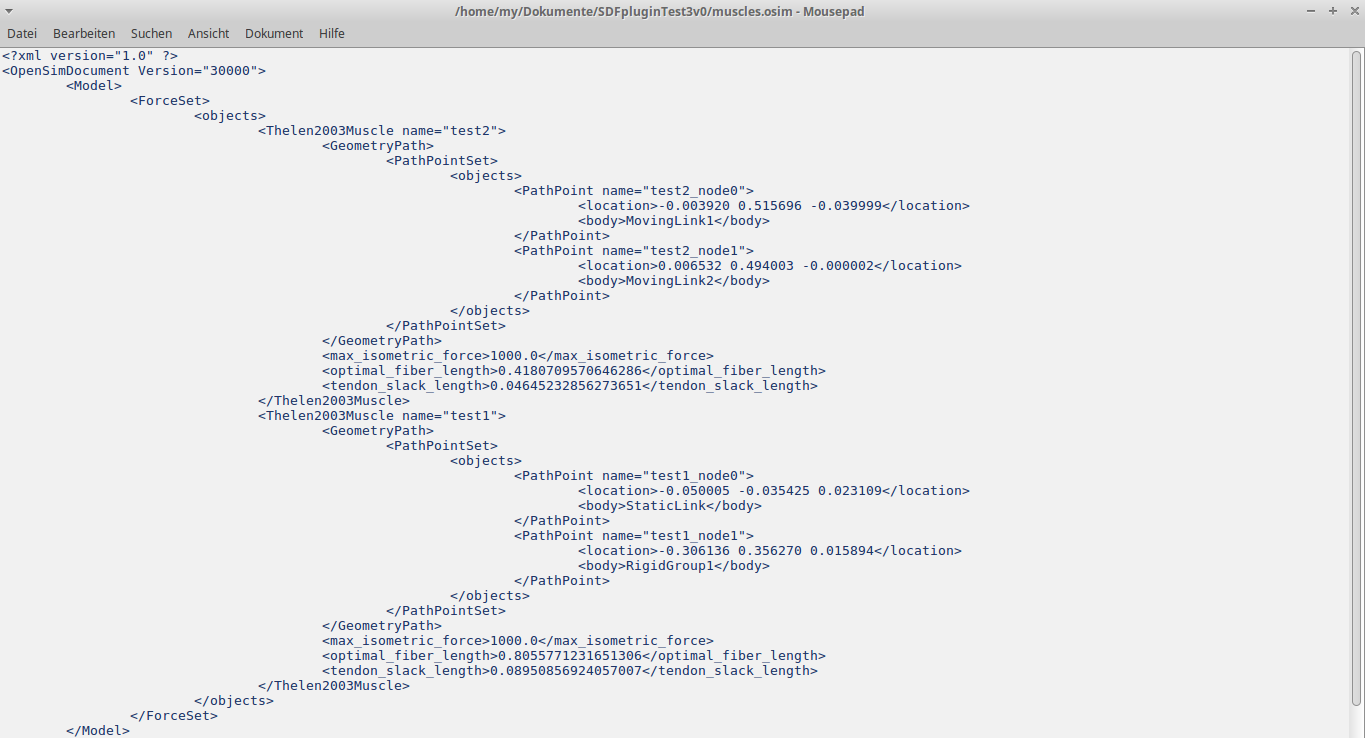
\includegraphics[width=0.95\textwidth] {figures/osim.png}
   \label{fig:osim}
 }\\
\subfigure[Edited model.sdf file that contains the MyoMuscle plug-in]{
   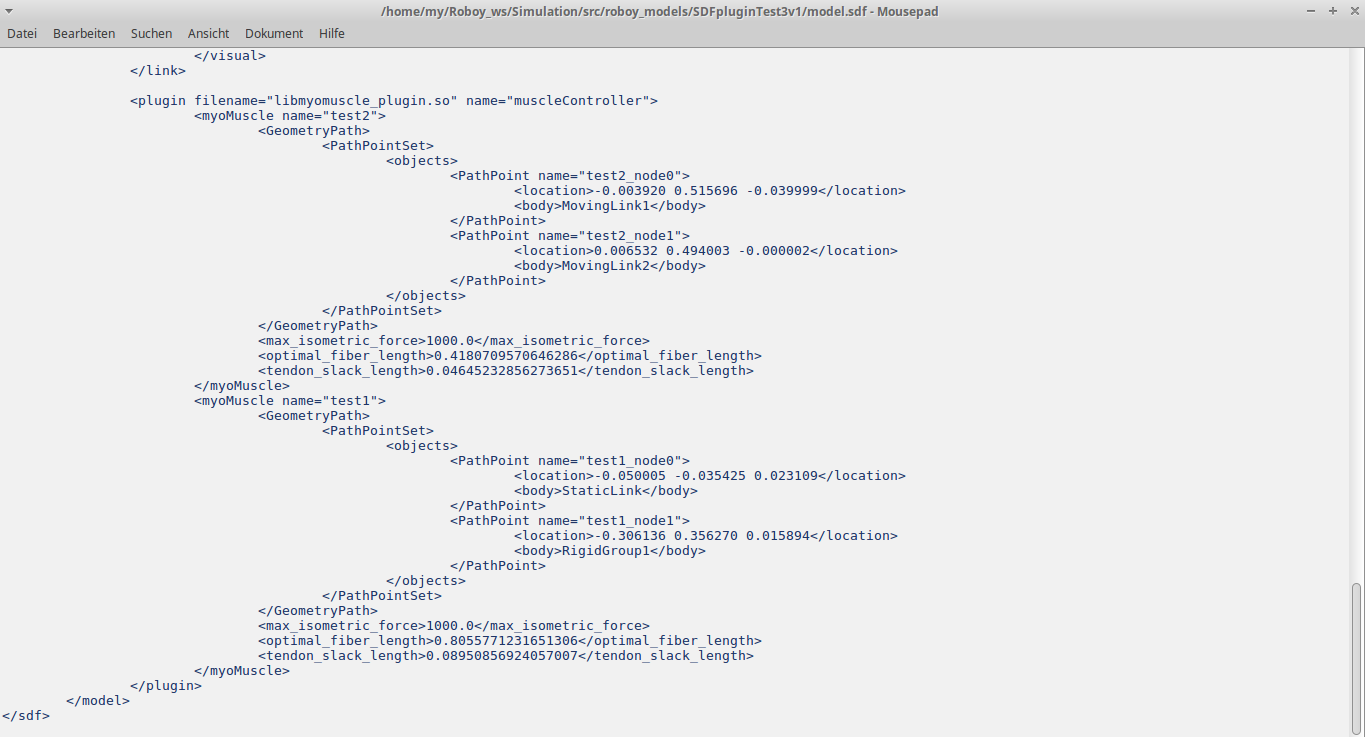
\includegraphics[width=0.95\textwidth]{figures/sdfplugin.png}
   \label{fig:sdf}
 }
 \caption{Adding the MyoMuscle plug-in to SDFormat files}
\end{figure}

